\section{Componenti e classi}
\label{componenti_classi}
\subsection{Romeo}
\label{pack_romeo}
	\subsubsection{Informazioni sul package}
	\label{info_romeo}
	\begin{figure}[!h]
		\centering
		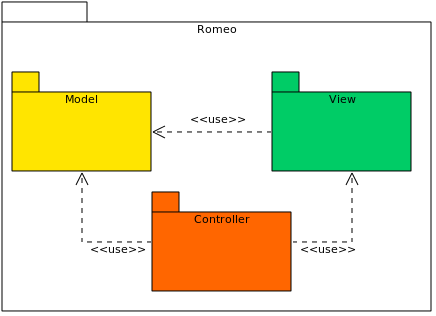
\includegraphics[scale=0.7]{./Content/Immagini/Romeo.png}
		\caption{Diagramma package \textsl{Romeo}}
		\label{MVC_Romeo}
	\end{figure}
	\subsubsection{Descrizione}
	\label{romeo_desc}
	Il package\glossario{} Romeo rappresenta il package\glossario{} globale del progetto.
	\\Le relazioni tra i package\glossario{} Model, View e Controller rappresentano le relazioni tipiche del design pattern\glossario{} MVC\glossario{}.
	\subsubsection{Package contenuti}
	\label{Romeo_contents}
	\begin{itemize}
		\item \hyperref[romeo::model]{Romeo::Model};
		\item \hyperref[romeo::view]{Romeo::View};
		\item \hyperref[romeo::controller]{Romeo::Controller}.
	\end{itemize}
	\subsubsection{Relazioni d'uso tra i componenti}
	I package\g{} contenuti nel package\g{} \project{}, rispettano il design pattern\g{} MVC\g{}. In particolare, il Model viene utilizzato dal Controller e dalla View; il primo per modificare i dati a seguito di un'interazione con l'utente, il secondo per visualizzarli. Inoltre, il Controller si relaziona anche con la View per aggiornare i dati.
	\pagebreak
	
\subsection{Romeo::Model}
\label{romeo::model}
	\subsubsection{Informazioni sul package}
	\label{info_model}
	\begin{figure}[!h]
		\centering
		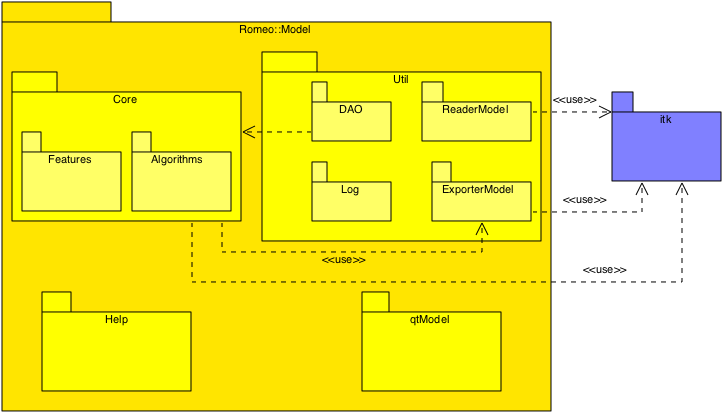
\includegraphics[scale=0.7]{./Content/Immagini/Romeo__Model.png}
		\caption{Diagramma package \textsl{Romeo::Mode}l}
		\label{comp_Romo::Model}
	\end{figure}
	\subsubsection{Descrizione}
	\label{info_model_descr}
	Package\glossario{} che rappresenta il componente model nell'architettura MVC\glossario{}.
	\subsubsection{Package contenuti}
	\label{contenuti_model}
	\begin{itemize}
		\item \hyperref[romeo::model::core]{Romeo::Model::Core};
		\item \hyperref[romeo::model::util]{Romeo::Model::Util};
		\item \hyperref[romeo::model::qtmodel]{Romeo::Model::qtModel};
		\item \hyperref[romeo::model::help]{Romeo::Model::Help}.
	\end{itemize}
	
\subsubsection{Relazioni d'uso tra i componenti}
In una visuale ad alto livello si nota che il package\g{} Core usa un package\g{} esterno, itk, per la manipolazione delle immagini con costrutti già esistenti e ben consolidati. Inoltre usa il package\g{} ExporterModel contenuto in Util. Il sotto-package\g{}  contenuto in Util usa il package\g{} Core, infine i package\g{} ReaderModel ed ExporterModel in Util usano il package\g{} esterno, itk, per la lettura e l'esportazione di immagini.
\\Infine il package\g{} qtModel viene utilizzato dalle classi del package\g{}  view.
\pagebreak	

%%%%%%%%%%%%%%%%%%%%%%%%%%%%%%%%%%%%%%%%%%%%%%%
%		CORE
%%%%%%%%%%%%%%%%%%%%%%%%%%%%%%%%%%%
	\subsection{Romeo::Model::Core}
	\label{romeo::model::core}
		\subsubsection{Informazioni sul package}
		\begin{figure}[!h]
			\centering
			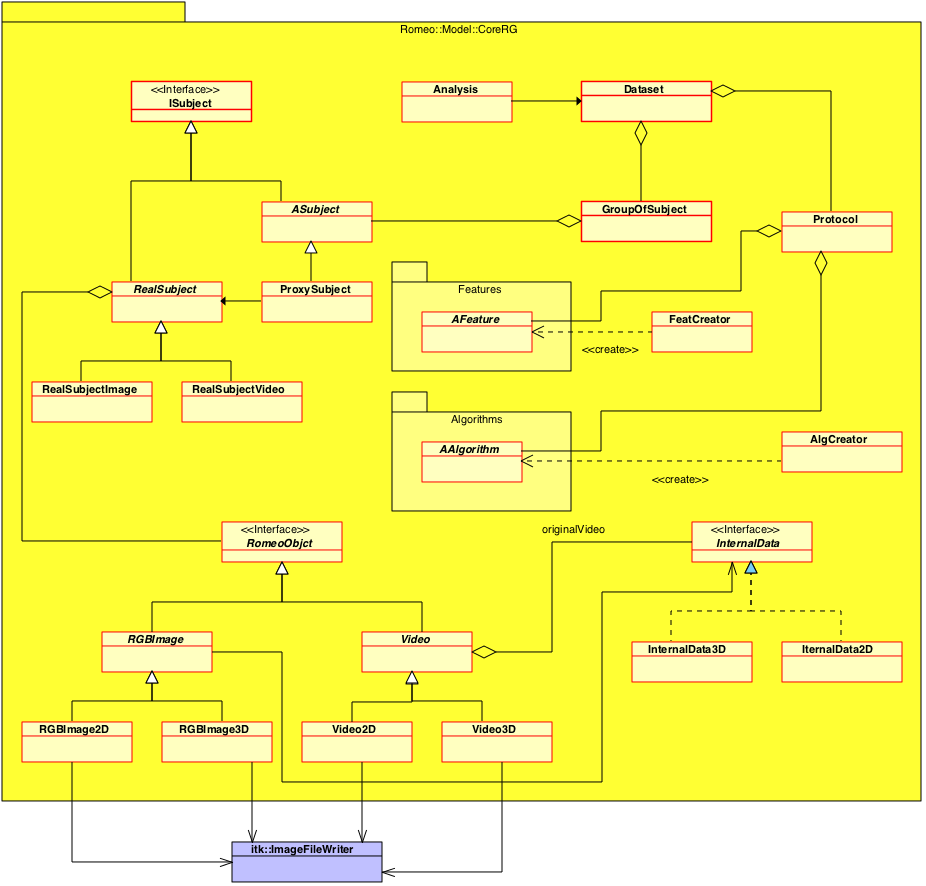
\includegraphics[width=1.1\linewidth]{./Content/Immagini/Romeo__Model__Core.png}
			\caption{Diagramma package \textsl{Romeo::Model::Core}}
		\end{figure}
		
		\subsubsection{Descrizione}
		Package\g{} contenente le classi rappresentanti le funzionalità principali del software. In questo package\g{} verrà utilizzato il design pattern\g{} Adapter, il quale consente di utilizzare alcune funzionalità offerte dalle librerie esterne.
		\subsubsection{Package contenuti}
		\begin{itemize}
				\item \hyperref[romeo::model::core::features]{Romeo::Model::Core::Features};
				\item \hyperref[romeo::model::core::algorithms]{Romeo::Model::Core::Algorithms}.
		\end{itemize}
		
		\subsubsection{Relazioni d'uso tra i componenti}
		\begin{itemize}
			\item La classe \textsl{ProxySubject} avrà un riferimento polimorfo ad un \textsl{RealSubject} e si occuperà di gestirne la creazione e le richieste;
			
			\item La classe \textsl{RealSubject} avrà un riferimento polimorfo ad un oggetto \textsl{RomeoObject};
			 
			\item La classe \textsl{RGBImage} avrà tre riferimenti polimorfi a \textsl{InternalData}, ognuno rappresentante un'immagine per ciascuno dei tre livelli di colore (Red, Green e Blue);
			
			\item La classe \textsl{Video} avrà un vettore di riferimenti ad oggetti \textsl{InternalData}, rappresentanti i \emph{frame} del video;
			
			\item La classe \textsl{GroupOfSubject} avrà una lista di riferimenti polimorfi alla classe \textsl{ASubjec}t, tanti quanti sono i Subject\g{} presenti nel gruppo;
			
			\item La classe \textsl{Dataset} avrà un riferimento alla classe \textsl{GroupOfSubject} e ad uno o più \textsl{Protocol};
			
			\item La classe \textsl{Analysis} avrà un riferimento alla classe \textsl{Dataset}, rappresentante il Dataset\g{} su cui eseguire l'analisi;
			
			\item Le classi \textsl{FeatCreator} e \textsl{AlgCreator} si occuperanno di creare le feature\g{} e gli algoritmi, tra quelli disponibili.
		\end{itemize}
		
		\subsubsection{Interfacce contenute}
		\label{int_contenute}
			\paragraph{\underline{ISubject}}
				
				\subparagraph{Descrizione:} definisce l’interfaccia comune per le classi \textsl{ASubject} e \textsl{RealSubjec}, fornisce un metodo per ottenere il formato interno per l’immagine del Subject\g{}.
				\\Rappresenta il componente Subject del design pattern\g{} Proxy.
				\label{core_isub}
				
				\subparagraph{Utilizzo:} viene utilizzata quando le componenti di Romeo\g{} necessitano di riferirsi a un Subject\g{} per ottenere il formato interno ad esso associato. 
				
				\subparagraph{Implementata da:}
					\begin{itemize}
						\item \hyperref[core_asub]{Romeo::Model::Core::Asubject};
						\item \hyperref[core_realsub]{Romeo::Model::Core::RealSubject}.
					\end{itemize}
					
				\subparagraph{Relazioni con altre classi:}
					\begin{itemize}
						\item \hyperref[RomeoObject]{Romeo::Model::Core::RomeoObject:} dipendenza uscente, i contratti forniti dall'interfaccia ISubject ritornano oggetti di tipo \textsl{RomeoObject}.
					\end{itemize}
			
			\pagebreak
		
			\paragraph{\underline{InternalData}}
			\label{internaldata}
			
				\subparagraph{Descrizione:} definisce l'interfaccia per accedere alle informazioni sulle dimensioni di un'immagine.
				\\Rappresenta il componente Target del design pattern\g{} Adapter.
				
				\subparagraph{Utilizzo:} viene utilizzata all'interno delle feature, ogni qualvolta ci si aspetta un' immagine generica.
				
				\subparagraph{Implementata da:}
					\begin{itemize}
						\item \hyperref[core_internal2d]{Romeo::Model::Core::InternalData2D};
						\item \hyperref[core_internal3d]{Romeo::Model::Core::InternalData3D}.
					\end{itemize}
					
					\subparagraph{Relazioni con altre classi:}
						\begin{itemize}
							\item \hyperref[]{Romeo::Model::Core::RGBImage:} relazione entrante, la classe \textsl{RGBImage} contiene tre riferimenti ad oggetti \textsl{InternalData} (red, green e blue).
									
							\item \hyperref[]{Romeo::Model::Core::Video:} relazione entrante, la classe \textsl{Video} contiene un vettore di oggetti \textsl{InternalData}, rappresentante i \emph{frame} del video.
							 
						\end{itemize}
					
				\paragraph{\underline{RomeoObject}}
				\label{romeoobject}
					
					\subparagraph{Descrizione:} intefaccia che rappresenta un generico dato da analizzare in Romeo\g{}.
					
					\subparagraph{Utilizzo:} viene utilizzato nei metodi delle feature e algoritmi per lavorare su un generico dato.
					
					\subparagraph{Implementata da:}
						\begin{itemize}
							\item \hyperref[]{Romeo::Model::Core::RGBImage};
							\item \hyperref[]{Romeo::Model::Core::Video}.
						\end{itemize}
					
				\subparagraph{Relazioni con altre classi:}
					\begin{itemize}				
						\item \hyperref[]{Sottoclassi di Romeo::Model::Core::AAlgorithm:} relazione entrante, 
						le sottoclassi di \textsl{AAlgorithm} necessitano di avere accesso al tipo \textsl{RomeoObject} per l'implementazione di alcuni metodi;
						
						\item \hyperref[]{Sottoclassi di Romeo::Model::Core::AFeature:} relazione entrante, le sottoclassi di \textsl{AFeature} necessitano di avere accesso al tipo \textsl{RomeoObject} per l'implementazione di alcuni metodi;
						
						\item \hyperref[]{Romeo::Model::Core::Analysis:} relazione entrante, la classe \textsl{
						} utilizza il tipo \textsl{RomeoObject} all'interno di alcuni metodi.
					\end{itemize}
		
		\subsubsection{Classi contenute}	
		\paragraph{\underline{ASubject}} 
		\label{core_asub}
			\subparagraph{Descrizione:} classe astratta che rappresenta un generico Subject\g{} con le relative proprietà \emph{Nome, Tipo del Subject\g{}, Immagine, Maschera e Data di creazione}.
			
			\subparagraph{Utilizzo:} viene utilizzata in seguito alla ricezione di un signal\g{} da
			 parte dei controller che necessitano di riferirsi ad uno o più oggetti di tipo \textsl{ASubject}.
			\\Inoltre viene utilizzata dalle classi DAO e dalla classe \textsl{GroupOfSubject}.
			
			\subparagraph{Eredita da:}
				\begin{itemize}
					\item \hyperref[core_isub]{Romeo::Model::Core::ISubject}.
				\end{itemize}
				
			\subparagraph{Ereditata da:}
				\begin{itemize}
					\item \hyperref[core_proxysub]{Romeo::Model::Core::ProxySubject}.
				\end{itemize}
				
			\subparagraph{Relazioni con alte classi:}
				\begin{itemize}
					\item \hyperref[group]{Romeo::Model::Core::GroupOfSubject:} relazione entrante, riferimenti all'insieme di Subject\g{} presenti nel gruppo;
					\item \hyperref[]{Romeo::Model::Util::DAO::SubjectDAO:} relazione entrante, la classe SubjectDAO necessità del tipo ASubject per la sua implementazione;
					\item \hyperref[]{Romeo::Controller::SubjectsController:} relazione entrante, la classe \textsl{SubjectsController} utilizza \textsl{ASubject} per visualizzare i Subject\g{} presenti nel sistema.
				\end{itemize}
			
		\paragraph{\underline{ProxySubject}} 
		\label{core_proxysub}
			\subparagraph{Descrizione:} classe che gestisce l’accesso ad un \textsl{RealSubject}, mantiene un riferimento che consente al proxy di accedere all’oggetto rappresentato \textsl{RealSubject}.
			\\Fornisce la stessa interfaaccia della classe \textsl{ASubject}, consentendo di utilizzare un oggetto \textsl{ProxySubject} quando è richiesto un oggetto \textsl{ASubject}.
			\\Rappresenta il componente Proxy del design pattern\g{} Proxy.
			
			\subparagraph{Utilizzo:} viene utilizzando quando è necessario creare un Subject\g{} all'interno di Romeo\g{}.
			
			\subparagraph{Eredita da:}
			\begin{itemize}
				\item \hyperref[core_asub]{Romeo::Model::Core::ASubject};
			\end{itemize}
			
			\subparagraph{Relazioni con altre classi:}
				\begin{itemize}
					\item \hyperref[realsubject]{Romeo::Model::Core::RealSubject:} relazione uscente, riferimento al \textsl{RealSubject} che il proxy sta gestendo;
					
					\item \hyperref[]{Romeo::Model::Core::RealSubjectImage:} relazione uscente, tipo dinamico del riferimento posseduto dal \emph{Proxy} quando sta gestendo un Subject\g{} 2D o 3D;
									
					\item \hyperref[]{Romeo::Model::Core.:RealSubjectVideo:} relazione uscente, tipo dinamico del riferimento posseduto dal \emph{Proxy} quando sta gestendo un Subject\g{} 2D-t o 3D-t; 
					
					\item \hyperref[]{Romeo::Util::DAO::SubjectDAO:} relazione entrante, la classe \textsl{SubjectDAO} necessità del tipo \textsl{ASubject} per la sua implementazione;
					
					\item \hyperref[]{Romeo::Controller::NewSubjectController:} relazione entrante, viene utilizzato il tipo \textsl{ProxySubject} per creare un nuovo Subject\g{} all'interno di Romeo\g{}.
					
				\end{itemize}
			
	\paragraph{\underline{RealSubject}}  
	\label{realsubject}
		
		\subparagraph{Descrizione:} classe astratta che caratterizza l’oggetto rappresentato dal \textsl{ProxySubject}, rappresenta un oggetto reale utilizzato dalla classe \textsl{ProxySubject}.
		\\Contiene la proprietà \emph{imageFormat}.
		\\Le sottoclassi rappresentano i componenti RealSubject del design pattern\g{} Proxy.
		
		\subparagraph{Utilizzo:} viene utilizzato dalla classe \textsl{ProxySubject}, la quale contiene un riferimento al \textsl{RealSubject} che sta gestendo.
		
		\subparagraph{Eredita da:}
			\begin{itemize}
				\item \hyperref[core_isub]{Romeo::Model::Core::ISubject}.
			\end{itemize}
			
		\subparagraph{Ereditata da:}
			\begin{itemize}
				\item \hyperref[core_realimage]{Romeo::Model::Core::RealSubjectImage};
				\item \hyperref[core_realvideo]{Romeo::Model::Core::RealSubjecVideo}.
			\end{itemize}
			
		\subparagraph{Relazioni con altre classi:}
			\begin{itemize}
				\item \hyperref[core_proxysub]{Romeo::Model::Core::ProxySubject:} relazione entrante, riferimento al \textsl{RealSubject} che il \textsl{ProxySubject} sta controllando;
				\item \hyperref[]{Romeo::Model::Core::RomeoObject:} relazione uscente, riferimento al formato interno rappresentante l'immagine del Subject\g{}.
			\end{itemize}
			
		\paragraph{\underline{RealSubjectImage}}
		\label{core_realimage}
			
			\subparagraph{Descrizione:} classe concreta che rappresenta un Subject\g{} nel formato bidimensionale (2D, 3D).
			\\Rappresenta il componente RealSubject del design pattern\g{} Proxy.
			
			\subparagraph{Utilizzo:} viene utilizzata dalla classe \textsl{ProxySubject} per ottenere l'oggetto di tipo \textsl{RomeoObject} che rappresenta l'immagine, quando il \textsl{ProxySubject} sta rappresentando un Subject\g{} 2D o 3D.
			
			\subparagraph{Eredita da:}
				\begin{itemize}
					\item \hyperref[core_realsub]{Romeo::Model::Core::RealSubject}.
				\end{itemize}
					
			\subparagraph{Relazioni con altre classi:}
				\begin{itemize}
					\item \hyperref[]{Romeo::Model::Core::ProxySubject:} relazione entrante, tipo dinamico del riferimento posseduto da un oggetto \textsl{ProxySubject}.
					
					\item \hyperref[RGBImage2D]{Romeo::Model::Core::RGBImage2D:} relazione uscente,  tipo dinamico del riferimento al formato interno dell'immagine del Subject\g{}, quando si sta rappresentando un Subject\g{}  2d;
					
					\item \hyperref[RGBImage3D]{Romeo::Model::Core::RGBImag3D:} relazione uscente, tipo dinamico del riferimento al formato interno della maschera del Subject\g{}, quando si sta rappresentando un Subject\g{} 3d.
				\end{itemize}

		\paragraph{\underline{RealSubjectVideo}}
		\label{core_realvideo
		}
			\subparagraph{Descrizione:} classe concreta che rappresenta un Subject\g{} di tipo 2D-t o 3D-t.
			\\Rappresenta il componente RealSubject del design pattern\g{} proxy.
			
			\subparagraph{Utilizzo:} viene utilizzata dalla classe \textsl{ProxySubject} per ottenere l'oggetto di tipo \textsl{RomeoObject} che rappresenta l'immagine, quando il \textsl{ProxySubject} sta rappresentando un Subject\g{} 2D-t o 3D-t.
			
			\subparagraph{Eredita da:}
				\begin{itemize}
					\item \hyperref[core_realsub]{Romeo::Model::Core::RealSubject}.
				\end{itemize}
				
			\subparagraph{Relazioni con altre classi:}
				\begin{itemize}
				
					\item \hyperref[]{Romeo::Model::Core::ProxySubject:} relazione entrante, tipo dinamico del riferimento posseduto da un oggetto \textsl{ProxySubject}.
				
					\item \hyperref[]{Romeo::Model::Core::Video2D:} relazione uscente, tipo dinamico del riferimento al formato interno dell'immagine del Subject\g{}, quando si sta rappresentando un Subject\g{} 2D-t;
					
					\item \hyperref[]{Romeo::Model::Core::Video3D:} relazione uscente, tipo dinamico del riferimento al formato interno dell'immagine del Subject\g{}, quando si sta rappresentando un Subject\g{} 3D-t;
				\end{itemize}

		\paragraph{\underline{GroupOfSubject}} 
		\label{group}
		
			\subparagraph{Descrizione:} classe che rappresenta un gruppo di Subject\g{} con le relative propietà: \emph{Nome del gruppo, tipo del gruppo, data di creazione e la lista di Subject\g{} presenti nel gruppo}.
			
			\subparagraph{Utilizzo:} viene utilizzata in seguito alla ricezione di un signal\g{} da parte dei controller che necessitano di riferirsi ad uno o più gruppi di Subject\g{}
			\\Inoltre viene utilizzata dalla classe \textsl{Dataset}, che contiene un riferimento al GroupOfSubject\g{} associato e dalle classi DAO.
			
			\subparagraph{Relazioni con altre classi:}
				\begin{itemize}
					\item \hyperref[dataset]{Romeo::Model::Core::Dataset:} relazione entrante, riferimento al Gruppo di Subject\g{} del Dataset\g{};
					
					\item \hyperref[]{Romeo::Model::Util::DAO::GroupDAO:} relazione entrante, la classe \textsl{GroupDAO} necessità del tipo per la sua implementazione;
					
					\item \hyperref[core_asub]{Romeo::Model::Core::ASubject:} relazione uscente, riferimento alla lista dei Subject\g{} presenti nel gruppo;
					
					\item \hyperref[]{Romeo::Controller::NewGroupController:} relazione entrante, necessita del tipo \textsl{GroupOfSubject} per la sua implementazione;
					
					\item \hyperref[]{Romeo::Controller::GroupsController:} realzione entrante, necessita del tipo \textsl{GroupOfSubject} per la sua implementazione.
				\end{itemize}

		\paragraph{\underline{Protocol}} 
		\label{protocol}

			\subparagraph{Descrizione:} classe che rappresenta un Protocol\g{} con le relative propietà: \emph{Nome, Tipo, Data di creazione, Lista di feature\g{} e Algoritmo di cluster\g{}}.
			
			\subparagraph{Utilizzo:} viene utilizzata in seguito alla ricezione di un signal\g{} da
			parte dei controller che necessitano di riferirsi ad uno o più Protocol\g{}.
			\\Inoltre viene utilizzata dalla classe \textsl{Dataset}, che contiene un riferimento ai Protocol\g{} associati, e dalle classi DAO.
			
			\subparagraph{Relazioni con altre classi:}
				\begin{itemize}
					\item \hyperref[dataset]{Romeo::Model::Core::Dataset:} relazione entrante, lista dei Protocol\g{} presenti nel Dataset\g{};
					
					\item \hyperref[]{Romeo::Model::Util::DAO::ProtocolDAO:} relazione entrante, la classe \textsl{ProtocolDAO} necessità del tipo per la sua implementazione;
					
					\item \hyperref[features::features]{Romeo::Model::Core::Features::AFeature:} relazione uscente, lista delle feature\g{} presenti nel Protocol\g{};
					
					\item \hyperref[algorithms::algorithms]{Romeo::Model::Core::Algorithms::AAlgorithm:} relazione uscente, riferimento all'algoritmo di cluster\g{} del Protocol\g{};
					
					\item \hyperref[]{Romeo::Controller::NewProtocolController:} realzione entrante, la classe necessita del tipo \textsl{Protocol} per la sua implementazione;
					
					\item \hyperref[]{Romeo::Controller::ProtocolsController:} realazione entrante, la classe necessita del tipo \textsl{Protocol} per la sua implementazione.
				\end{itemize}
			
		\paragraph{\underline{Dataset}} 
		\label{dataset}
			
			\subparagraph{Descrizione:} classe che rappresenta un Dataset\g{} con le relative proprietà: \textit{Nome}, \textit{Tipo}, \textit{Data di creazione}, \textit{Gruppo di Subject\g{}} e \textit{Protocol\g{}}.

			\subparagraph{Utilizzo:} viene utilizzata in seguito alla ricezione di un signal\g{} da parte dei controller che necessitano di riferirsi ad uno o più Dataset\g{}.			
			\\Inoltre viene utilizzata dalla classe \textsl{Analysis}, che contiene un riferimento al Dataset\g{} associato all'analisi, e dalle classi DAO.
			
			\subparagraph{Relazioni con altre classi:}
				\begin{itemize}
					\item \hyperref[analysis]{Romeo::Model::Core::Analysis:} relazione entrante, riferimento al Dataset\g{} su cui eseguire l'analisi;
				
					\item \hyperref[]{Romeo::Model::Util::DAO::DatasetDAO} relazione entrante, la classe \textsl{DatasetDAO} necessità del tipo \textsl{Dataset} per la sua implementazione;
					
					\item \hyperref[group]{Romeo::Model::Core::GroupOfSubject:} relazione uscente, gruppo di Subject\g{} associato al Dataset\g{};
					
					\item \hyperref[protocol]{Romeo::Model::Core::Protocol:} relazione uscente, lista dei Protocol\g{} presenti nel Dataset\g{};
					
					\item \hyperref[]{Romeo::Controller::NewDatasetController:} relazione entrante, la classe \textsl{NewDatasetController} necessita del tipo \textsl{Dataset} per la sua implementazione;
					
					\item \hyperref[]{Romeo::Controller::DatasetsController:} relazione entrante, la classe \textsl{DatasetsController} necessita del tipo \textsl{Dataset} per la sua implementazione.
	
				\end{itemize}

		\paragraph{\underline{Analysis}} 
		\label{analysis}
			\subparagraph{Descrizione:} classe che rappresenta un' analisi con le relative proprietà: \emph{Subject\g{} da analizzare, Directory dei risultati, Feature\g{} di cui salvare i risultati, Feature\g{} di cui visualizzare i risultati e Data di creazione}.

			\subparagraph{Contesto di utilizzo:} viene utilizzata dalla classe \textsl{AnalysisController}, alla ricezione di un signal\g{} per l'avvio di una nuova analisi.
		
		\subparagraph{Eredita da:}
			\begin{itemize}
				\item  Qt::QThread.
			\end{itemize}
			
		\subparagraph{Relazioni con altre classi:}
			\begin{itemize}
				\item \hyperref[]{Romeo::Model::Uitl::DAO::AnalysisDAO:} relazione entrante, la classe \textsl{AnalysisDAO} necessità del tipo \textsl{Analysis} per la sua implementazione;
				\item \hyperref[dataset]{Romeo::Model::Core::Dataset:} relazione uscente, riferimento al Dataset\g{} su cui eseguire l'analisi;
				\item \hyperref[]{Romeo::Model::Core::RomeoObject:} realzione uscente, necessità del tipo \textsl{RomeoObject} per la sua implementazione.
			\end{itemize}

		\paragraph{\underline{FeatCreator}} 
		\label{featC}
		
			\subparagraph{Descrizione:} classe Factory avente la responsibilità di creare un oggetto della classe Romeo::Model::Core::Features::AFeature, che rappresenta un'istanza della feature\glossario{} da creare.
			\\Rappresenta il componente Factory del design pattern\g{} Factory.
			\\A seconda dei parametri e nome della Feature\g{} passati, crea un oggetto rispetto ad un altro.
			
			\subparagraph{Utilizzo: } viene utilizzata in seguito alla ricezione di un signal\g{} da parte dei controller che necessitano di utilizzare un oggetto di tipo \textsl{Romeo::Model::Core::Algorithms::AFearure}.
			\\A seconda dei parametri e nome della feature\g{} passati, crea un oggetto rispetto ad un altro.
			
			\subparagraph{Relazioni con altre classi:}
				\begin{itemize}
					\item Sottoclassi di \hyperref[features::features]{Romeo::Model::Core::Features::AFeature:} relazione uscente, la classe FeatCreator si occupa di creare le istanze delle varie Feature\g{} disponibili;
					
					\item \hyperref[AFeature]{Romeo::Model::Core::Features::AFeature:} relazione uscente, tipo statico di una feature\g{} creata dalla classe FeatCreator;
					
					\item \hyperref[]{Romeo::Controller::NewProtocolController:} relazione entrante, la classe \textsl{NewProtocolController} necessita del tipo \textsl{FeatCreator} per la sua implementazione;
					
					\item \hyperref[]{Romeo::Controller::ProtocolsController:} relazione entrante, la classe \textsl{ProtocolsController} necessita del tipo \textsl{FeatCreator} per la sua implementazione;
					
					\item \hyperref[]{Romeo::Controller:AnalysisController:} relazione entrante, la classe \textsl{AnalysisController} necessita del tipo \textsl{FeatCreator} per la sua implementazione.
				\end{itemize}
		
		\paragraph{\underline{AlgCreator}} 
		\label{algC}
			
			\subparagraph{Descrizione:} classe Factory avente la responsabilità di creare un oggetto di tipo \textsl{Romeo::Model::Core::Algorithms::AAlgorithm}, che rappresenta un' instanza dell' algoritmo da creare.
			\\Rappresenta il componente Factory del design pattern\g{} Factory.
			
			\subparagraph{Utilizzo:} viene utilizzata in seguito alla ricezione di un signal\g{} da parte dei controller che necessitano di utilizzare un oggetto di tipo \textsl{Romeo::Model::Core::Algorithms::AAlgorithm}.
			\\A seconda dei parametri e nome dell’ algoritmo di Cluster\g{} passati, crea un oggetto rispetto ad un altro.
			
			\subparagraph{Relazioni con altre classi:}
				\begin{itemize}
					\item Sottoclassi di \hyperref[AAlgorithm]{Romeo::Model::Core::Algorithms::AAlgorithm:} relazione uscente, la classe AlgCreator si occupa di creare le istanze dei vari Algoritmi di Cluster\g{} disponibili;
				
					\item \hyperref[AAlgorithm]{Romeo::Model::Core::Algorithms::AAlgorithm;} relazione uscente, tipo statico di un algoritmo creato dalla classe Factory;
					
					\item \hyperref[]{Romeo::Controller::NewProtocolController:} relazione entrante, la classe \textsl{NewProtocolController} necessita del tipo \textsl{AlgCreator} per la sua implementazione;
					
					\item \hyperref[]{Romeo::Controller::ProtocolsController:} relazione entrante, la classe \textsl{ProtocolsController} necessita del tipo \textsl{AlgCreator} per la sua implementazione;
					
					\item \hyperref[]{Romeo::Controller:AnalysisController:} relazione entrante, la classe \textsl{AnalysisController} necessita del tipo \textsl{AlgCreator} per la sua implementazione.
				\end{itemize}
			
		\paragraph{\underline{InternalData2D}}
		\label{core_internal2d}
		
			\subparagraph{Descrizione:} classe che implementa i contratti definiti da InternalData e rappresenta il formato interno bidimensionale sul quale operare. Implementa il design pattern Adapter e adatta la classe itk::Image della libreria ITK\g{}. Rappresenta la componente Adapter dell'omonimo design pattern\g{}.
			
			\subparagraph{Utilizzo:} viene utlizzata nelle feature\g{} come parametro di input da elaborare e rappresenta i signoli canali nelle immagini in formato RGB.
			
			\subparagraph{Eredita da:}
				\begin{itemize}
					\item \hyperref[internaldata]{Romeo::Model::Core::InternalData}.
				\end{itemize}
				
			\subparagraph{Relazioni con altre classi:}
				\begin{itemize}
					\item \hyperref[]{Romeo::Model::Core::RGBImage2D:} relazione entrante, tipo dinamico del riferimento posseduto dalla classe \textsl{RGBImage2D};
					
					\item \hyperref[]{Romeo::Model::Core::Video2D:} relazione entrante, tipo dinamico del vettore posseduto dalla classe \textsl{Video2D};
					
					\item \hyperref[]{Romeo::Model::Core::Algorithms::AAlgorithm:} relazione entrante, le classi rappresentanti gli algoritmi utilizzano il tipo \textsl{InternalData2D} nella loro implementazione;
					
					\item \hyperref[]{Romeo::Model::Core::Features::AFeature:} relazione entrante, le classi rappresentanti le featur utilizzano il tipo \textsl{InternalData2D} nella loro implementazione.
				\end{itemize}


		\paragraph{\underline{InternalData3D}}
		\label{core_internal3d}
		\subparagraph{Descrizione:} classe che rappresenta il formato interno per un'immagine di tipo 3D.
		\\Classe che \lq\lq{}adatta\rq\rq{} la classe itk::image fornita dalla libreria esterna ITK\g{}.
		\\Rappresenta il componente Adapter del design pattern\g{} Adapter.
					
					\subparagraph{Utilizzo:} viene utlizzata nelle feature\g{} come parametro di input da elaborare e rappresenta i signoli canali nelle immagini in formato RGB.
					
					\subparagraph{Eredita da:}
						\begin{itemize}
							\item \hyperref[internaldata]{Romeo::Model::Core::InternalData}.
						\end{itemize}
						
					\subparagraph{Relazioni con altre classi:}
						\begin{itemize}
							\item \hyperref[]{Romeo::Model::Core::RGBImage3D:} relazione entrante, tipo dinamico del riferimento posseduto dalla classe \textsl{RGBImage2D};
							
							\item \hyperref[]{Romeo::Model::Core::Video3D:} relazione entrante, tipo dinamico del vettore posseduto dalla classe \textsl{Video2D};
							
							\item \hyperref[]{Romeo::Model::Core::Algorithms::AAlgorithm:} relazione entrante, le classi rappresentanti gli algoritmi utilizzano il tipo \textsl{InternalData3D} nella loro implementazione;
							
							\item \hyperref[]{Romeo::Model::Core::Features::AFeature:} relazione entrante, le classi rappresentanti le featur utilizzano il tipo \textsl{InternalData3D} nella loro implementazione.
						\end{itemize}
						
		\paragraph{\underline{RGBImage}}
		\label{RGBImage}
			\subparagraph{Descrizione:} classe astratta che rappresenta un'immagine RGB, composta da tre livelli di colore \textit{red, green} e \textit{blue}. Definisce dei contratti per l'accesso ai tre livelli di colore, per la loro scomposizione e fusione.
			
			\subparagraph{Utilizzo:} viene utilizzata quando una feature\g{}  deve essere applicata ad un immagine e non ad un video.
			\\Inoltre viene utilizzata per salvare le informazioni riguardanti il colore dell'immagine, che altrimenti sarebbe in scala di grigi.
			
			\subparagraph{Eredita da:}
				\begin{itemize}
					\item \hyperref[]{Romeo::Model::Core::RomeoObject}.
				\end{itemize}
				
			\subparagraph{Realazioni con altre classi:}
				\begin{itemize}
					
					\item \hyperref[]{Romeo::Model::Core::InternalData:} relazione uscente, la classe \textsl{RGBImage} contiene tre riferimenti ad oggetti di tipo \textsl{InternalData} (red, green e blue);
					
					\item \hyperref[]{Romeo::Model::Core::Analysis:} relazione entrante, la classe \textsl{Analysis} necessita del tipo \textsl{RGBImage} per la sua implementazione;
					
					\item \hyperref[]{Romeo::Model::Core::Algorithms::AAlgorihm:} relazione entrante, la classe \textsl{AAlgorithm} necessità del tipo \textsl{RGBImage} per la sua implementazione;
					
					\item \hyperref[]{Romeo::Model::Core::Features::AFeature:} relazione entrante, la classe \textsl{AFeature} necessita del tipo \textsl{RGBImage} per la sua implementazione.
					
				\end{itemize}
						
		\paragraph{\underline{RGBImage2D}}
		\label{RGBImage2D}
			
			\subparagraph{Descrizione:} classe che rappresenta un immagine bidimensionale, a colori in Romeo\g{}
			\\Classe che \lq\lq{}adatta\rq\rq{} la classe itk::image fornita da itk.
			\\Rappresenta il componente Adapter del design pattern\g{} Adapter.
			
			\subparagraph{Utilizzo:} viene utilizzata dalle feature\g{} che elaborano immagini bidimensionali.
			\\Inoltre racchiude in se le informazioni sul colore delle immagini importate.
			
			\subparagraph{Eredita da:}
				\begin{itemize}
					\item \hyperref[RGBImage]{Romeo::Model::Core::RGBImage}.
				\end{itemize}
				
			\subparagraph{Relazioni con altre classi:}
				\begin{itemize}
					\item \hyperref[]{Romeo::Model::Core::RealSubjectImage:} relazione entrante, tipo dinamico del riferimento posseduto dalla classe;
					\item \hyperref[]{Romeo::Model::Core::Video2D:} relazione entrante, tipo dinamico del vettore di immagini RGB;
				\end{itemize}
				
		\paragraph{\underline{RGBImage3D}}
		\label{RGBImage3D}
			
				\subparagraph{Descrizione:} classe che rappresenta un immagine tridimensionale, a colori in Romeo\g{}
						\\Classe che \lq\lq{}adatta\rq\rq{} la classe itk::image fornita da itk.
						\\Rappresenta il componente Adapter del design pattern\g{} Adapter.
						
						\subparagraph{Utilizzo:} viene utilizzata dalle feature\g{} che elaborano immagini tridimensionali.
						\\Inoltre racchiude in se le informazioni sul colore delle immagini importate 
						
						\subparagraph{Eredita da:}
							\begin{itemize}
								\item \hyperref[RGBImage]{Romeo::Model::Core::RGBImage}.
							\end{itemize}
							
						\subparagraph{Relazioni con altre classi:}
							\begin{itemize}
								\item \hyperref[]{Romeo::Model::Core::RealSubjectImage:} relazione entrante, tipo dinamico dei riferimenti posseduti dalla classe;
								\item \hyperref[]{Romeo::Model::Core::Video3D:} relazione entrante, tipo dinamico del vettore di immagini RGB;
							\end{itemize}
				
		\paragraph{\underline{Video}}

			
			\subparagraph{Descrizione:} classe astratta che rappresenta la classe base di tutti i video in Romeo\g{}.
			\\È composta da un vettore di oggetti di tipo \textsl{InternalData}.
			
			\subparagraph{Utilizzo:} viene utilizzata dalle Feature\g{} dinamiche quando ci si aspetta un video generico.
			
			\subparagraph{Eredita da:}
				\begin{itemize}
					\item \hyperref[]{Romeo::Model::Core::RomeoObject}.
				\end{itemize}
				
			\subparagraph{Relazioni con altre classi:}
				\begin{itemize}
					\item \hyperref[]{Romeo::Model::Core::InternalData:} relazione uscente, vettore di immagini rappresentante i vari \emph{frame} del video;
					
					\item \hyperref[]{Romeo::Model::Core::Analysis:} relazione entrante, la classe \textsl{Analysis} necessita del tipo \textsl{Video} per la sua implementazione;
										
					\item \hyperref[]{Romeo::Model::Core::Algorithms::AAlgorihm:} relazione entrante, la classe \textsl{AAlgorithm} necessità del tipo \textsl{Video} per la sua implementazione;
					
					\item \hyperref[]{Romeo::Model::Core::Features::AFeature:} relazione entrante, la classe \textsl{AFeature} necessita del tipo \textsl{Video} per la sua implementazione.
					
				\end{itemize}
		
		\paragraph{\underline{Video2D}}
		\label{video2d}
		
			\subparagraph{Descrizione;} classe concreta che rappresenta un video bidimensionale in Romeo\g{}.
			
			\subparagraph{Utilizzo:} viene utlizzata delle classi rappresentanti le Feature\g{} dinamiche 2D come dato da processare.
			
			\subparagraph{Eredita da:}
				\begin{itemize}
					\item \hyperref[]{Romeo::Model::Core::Video}.
				\end{itemize}
				
			\subparagraph{Relazioni con altre classi:}
				\begin{itemize}
					\item \hyperref[]{Romeo::Modeo:::Core::RealSubjectVideo:} relazion entrante, tipo dinamico del vettore posseduto
				\end{itemize}
			
		\paragraph{\underline{Video3D}}
		
			\subparagraph{Descrizione:} classe concreta che rappresenta un video bidimensionale in Romeo\g{}.
			
			\subparagraph{Utilizzo:} viene utlizzata dalle Feature\g{} dinamiche 3D come dato da processare.
			
			\subparagraph{Eredita da:}
				\begin{itemize}
					\item \hyperref[]{Romeo::Model::Core::Video}.
				\end{itemize}
				
			\subparagraph{Relazioni con altre classi:}
				\begin{itemize}
					\item \hyperref[]{Romeo::Model::Core::RealSubjectVideo:} relazione entrante, tipo dinamico del vettore posseduto dalla classe.
				\end{itemize}

%%%%%%%%%%%%%%%%%%%%%%%%%%%%%%%%%%%%%%%%%%%%%
	\subsection{Romeo::Model::Core::Features}
	\label{romeo::model::core::features}
		\subsubsection{Informazioni sul package}
		\begin{figure}[!h]
			\centering
			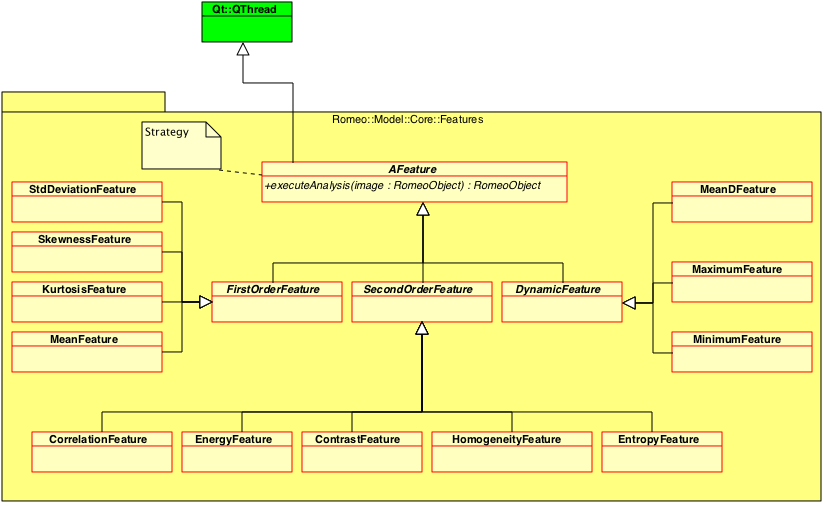
\includegraphics[width=1.1\linewidth]{./Content/Immagini/Romeo__Model__Core__Adapters__Features.png}
			\caption{Diagramma package \textsl{Romeo::Model::Core::Features}}
		\end{figure}	
		
		\subsubsection{Descrizione}
		Package\g{} contenente le classi che permettono al model di utilizzare le features\glossary{} previste nei requisiti. Le classi di questo package\g{} sono implementate usando il design pattern\g{} Strategy.
		
		\subsubsection{Classi contenute}
		\paragraph{\underline{AFeature}}
		\label{features::features} 
		
			\subparagraph{Descrizione:} classe astratta che rappresenta una generica feature\g{}. \\Definisce dei contratti per l’esecuzione delle feature\g{}, che dovranno essere implementati dalle sue sottoclassi. Rappresenta la componente Strategy dell’omonimo design pattern\g{}.
			
			\subparagraph{Utilizzo:} fornisce i metodi per l’esecuzione di una feature\g{} su un immagine bidimensionale o tridimensionale.
			
			\subparagraph{Eredita da:}
				\begin{itemize}
					\item Qt::QThread.
				\end{itemize}
				
			\subparagraph{Ereditata da:}
				\begin{itemize}
					\item \hyperref[features:fistorder]{Romeo::Model::Core::Adapters::Features::FirstOrder};
					\item \hyperref[features:secondorder]{Romeo::Model::Core::Adapters::Features::SecondOrder};
					\item \hyperref[features::dynamic]{Romeo::Model::Core::Adapters::Features::DynamicFeature}.
				\end{itemize}
				
			\subparagraph{Relazioni con altre classi:}
				\begin{itemize}
					\item \hyperref[protocol]{Romeo::Model::Core::Protocol:} relazione entrante, lista delle Feature\g{} presenti nel Protocol\g{};
				
					\item \hyperref[featC]{Romeo::Model::Core::FeatCreator:} relazione entrante, tipo statico di una Feature\g{} creata dalla classe Factory;
					
					\item \hyperref[]{Romeo::Model::Util::DAO::FeatureDAO:} relazione entrante, la classe FeatureDAO necessità del tipo FeatureDAO per la sua implementazione.

					
				\end{itemize}
		
		\paragraph{\underline{FirstOrder}}
		\label{features:fistorder}
		
			\subparagraph{Descrizione:} classe astratta che rappresenta una generica feature\g{} del primo ordine. Deriva da \textsl{AFeature} e rimane astratta perchè non implemente i contratti di quest'ultima.
			\\Tale classe è caratterizzata da un campo dati \textit{window size}. 
			\\Le sue sottoclassi rappresenteranno le componenti ConcreteStrategy del design pattern\g{} Strategy. 
			
			\subparagraph{Utilizzo:} viene utilizzata durante un’analisi recuperare le informazioni sulla dimensione della finetra, la lista dei parametri e il tipo della feature\g{}.
			
			\subparagraph{Eredita da:}
				\begin{itemize}
						\item \hyperref[features::features]{Romeo::Model::Core::Features::AFeature}
				\end{itemize}
				
			\subparagraph{Ereditata da:}
				\begin{itemize}
					\item \hyperref[]{Romeo::Model::Core::Features::StdDeviationFeature};
					\item \hyperref[]{Romeo::Model::Core::Features::SkewnessFeature};
					\item \hyperref[]{Romeo::Model::Core::Features::KurtosisFeature};
					\item \hyperref[]{Romeo::Model::Core::Features::MeanFeature}.
				\end{itemize}
				
			\subparagraph{Relazioni con altre classi:}
				\begin{itemize}
					\item \hyperref[]{Romeo::Model::Core::FeatCreator:} relazione entrante, la classe \textsl{FeatCreator} utilizza il tipo \textsc{FirstOrder} per la sua implementazione. 
				\end{itemize}
							
		\paragraph{\underline{SecondOrder}}
		\label{features:secondorder}
		
			\subparagraph{Descrizione:} classe astratta che rappresenta una generica feature\g{} del secondo ordine. Deriva da \textsc{AFeature} e rimane astratta perchè non implementa i contratti di quest'ultima. Le sue sottoclassi rappresentano le componente ConcreteStrategy del design pattern\g{} Strategy.
			
			\subparagraph{Utilizzo:} viene utilizzata durante un’analisi recuperare le informazioni sulla dimensione della finetra, la lista dei parametri e il tipo della feature\g{}.
			
			\subparagraph{Eredita da:}
				\begin{itemize}
					\item \hyperref[features::features]{Romeo::Model::Core::Features::AFeature}.
				\end{itemize}
				
			\subparagraph{Ereditata da:}
				\begin{itemize}
					\item \hyperref[]{Romeo::Model::Core::Features::CorrelationFeature};
					\item \hyperref[]{Romeo::Model::Core::Features::EnergyFeature};
					\item \hyperref[]{Romeo::Model::Core::Features::ContrastFeature};
					\item \hyperref[]{Romeo::Model::Core::Features::HomegeneityFeature};
					\item \hyperref[]{Romeo::Model::Core::Features::EntropyFeature}.
				\end{itemize}
				
			\subparagraph{Relazioni con altre classi:}
						\begin{itemize}
							\item \hyperref[]{Romeo::Model::Core::FeatCreator:} relazione entrante, la classe \textsl{FeatCreator} utilizza il tipo \textsl{SecondOrder} per la sua implementazione. 
						\end{itemize}
			
		\paragraph{\underline{DynamicFeature}}
		\label{features::dynamic}
		
			\subparagraph{Descrizone:} classe astratta che rappresenta una generica feature\g{} dinamica. Deriva da \textsl{AFeature} e rimane astratta perchè non implementa i contratti di quest'ultima. Le sue sottoclassi rappresenteranno le componenti ConcreteStrategy del design pattern\g{} Strategy.
			
			\subparagraph{Utilizzo:} viene utilizzata durante un’analisi recuperare la lista dei parametri e il tipo della feature\g{}.
			
			\subparagraph{Eredita da:}
				\begin{itemize}
					\item \hyperref[features::features]{Romeo::Model::Core::Features::AFeature}.
				\end{itemize}
				
			\subparagraph{Ereditata da:}
				\begin{itemize}
					\item \hyperref[]{Romeo::Model::Core::Features::MeanDFeature};
					\item \hyperref[]{Romeo::Model::Core::Features::MaximumFeature};
					\item \hyperref[]{Romeo::Model::Core::MinimumFeature}.
				\end{itemize}
				
			\subparagraph{Relazioni con altre classi:}
				\begin{itemize}
					\item \hyperref[]{Romeo::Model::Core::FeatCreator:} relazione entrante, la classe \textsl{FeatCreator} utilizza il tipo \textsc{DynamicFeature} per la sua implementazione. 
				\end{itemize}
			
			
	\pagebreak

%%%%%%%%%%%%%%%%%%%%%%%%%%%%%%%%%%%%			
	\subsection{Romeo::Model::Core::Algorithms}
	\label{romeo::model::core::algorithms}
	
		\subsubsection{Informazioni sul package}
		\begin{figure}[!h]
			\centering
			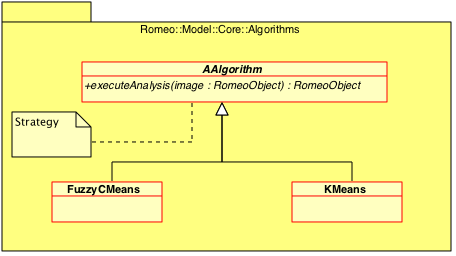
\includegraphics[width=0.9\linewidth]{./Content/Immagini/Romeo__Model__Core__Adapters__Algorithms.png}
			\caption{Diagramma package \textsl{Romeo::Model::Core::Algorithms}}
		\end{figure}		
		
		\subsubsection{Descrizione}
		Package\g{} contenente le classi che permettono al model di utilizzare gli algoritmi di clustering\g{} previsti nei requisiti.	
		Le classi di questo pacakge\g{} sono implementate utilizzando il design pattern\g{} Strategy.	
		
		
		\subsubsection{Classi contenute}
		\paragraph{\underline{AAlgorithm}}
		\label{algorithms::algorithms} 
		
			\subparagraph{Descrizione:} classe astratta che rappresenta un generico algoritmo di clustering\g{}, secondo il design pattern\g{} Strategy. Definisce dei contratti per l’esecuzione degli algoritmi, che dovranno essere implementati dalle sue sottoclassi.
			\\Rappresenta il componente Strategy dell'ononimo design pattern\g{}.
			
			\subparagraph{Utilizzo:} fornisce i metodi per l’esecuzione di un algoritmo di clustering\g{} su un immagine bidimensionale o tridimensionale.
			
			\subparagraph{Ereditata da:}
				\begin{itemize}
					\item \hyperref[algorithms:fuzzycmeans]{Romeo::Model::Core::Algorithms::FuzzyCMeans};
					\item \hyperref[algorithms::kmeans]{Romeo::Model::Core::Algorithms::KMeans}.
				\end{itemize}
				
			\subparagraph{Relazioni con altre classi:}
				\begin{itemize}
					\item \hyperref[protocol]{Romeo::Model::Core::Protocol:} relazione entrante riferimento all'algoritmo contenuto dal Protocol\g{};
					
					\item \hyperref[algC]{Romeo::Model::Core::AlgCreator:} relazione entrante, tipo statico di un algoritmo di cluster\g{} creato dalla classe Factory;
					
					\item \hyperref[]{Romeo::Model::Core::RomeoObject:} relazione uscente, il metodo executeAnalysis lavora su un oggetto di tipo statico \textsl{RomeoObject};
					
					\item \hyperref[]{Romeo::Model::Core::RGBImage:} relazione uscente, la classe \textsl{AAlgorithm} utilizza il tipo \textsc{RGBImage} per la sua implementazione;
					
					\item \hyperref[RGBImage2D]{Romeo::Model::Core::RGBImage2D:} relazione uscente, la classe \textsl{AAlgorithm} utilizza il tipo \textsl{RGBImage2D} per eseguire un' analisi su un' immagine 2D;
					
					\item \hyperref[RGBImage3D]{Romeo::Model::Core::RGBImage3D:} relazione uscente, la classe \textsl{AAlgorithm} utlizza il tipo \textsc{RGBImage3D} per eseguire un' analisi su un' immagine 3D;
					
					\item \hyperref[]{Romeo::Model::Core::Video:} relazione uscente, la classe \textsl{AAlgorithm} utilizza il tipo \textsc{Video} per la sua implementazione;
					
					\item \hyperref[]{Romeo::Model::Core::Video2D:} relazione uscente, la classe \textsl{AAlgorithm} utilizza il tipo \textsl{Video2D} per l' analisi su Video in formato 2D;
					
					\item \hyperref[]{Romeo::Model::Core::Video3D:} relazione uscente, la classe \textsc{AAlgorithm} utilizza il tipo \textsl{Video3D} per l' analisi su Video in formato 3D;
					
					\item \hyperref[]{Romeo::Model::Util::DAO::AlgorithmDAO:} relazione entrante, la classe AlgorithmDAO necessità del tipo AAlgorithm per la sua implementazione.
					
				\end{itemize}
												
		\paragraph{\underline{FuzzyCMeans}}
			\label{algorithms:fuzzycmeans}
			
				\subparagraph{Descrizione:} classe che implementa l’algoritmo di clustering\g{} FuzzyCMeans.
				\\Rappresenta il componente ConcreteStrategy del design pattern\g{} Strategy.
				
				\subparagraph{Utilizzo:} viene utilizzata durante un’analisi per applicare l’algoritmo a un Dataset\g{}.
				
				\subparagraph{Eredita da:}
					\begin{itemize}
						\item \hyperref[algorithms::algorithms]{Romeo::Model::Core::Algorithms::AAlgorithm}.
					\end{itemize}
					
				\subparagraph{Relazioni con altre classi:}
					\begin{itemize}
						\item \hyperref[]{Romeo::Model::Core::AlgCreator:} relazione entrante, la classe AlgCreator necessità di vedere il tipo \textsl{FuzzyCMeans} per la sua implementazione.
					\end{itemize}
		
		\paragraph{\underline{KMeans}}
		\label{algorithms::kmeans}
		
			\subparagraph{Descrizione:} classe che implementa l’algoritmo di clustering\g{} K-Means.
			\\Rappresenta il componente ConcreteStrategy del design pattern\g{} Strategy.
			
			\subparagraph{Utilizzo:} viene utilizzata durante un’analisi per applicare l’algoritmo a un Dataset\g{}.
			
			\subparagraph{Eredita da:}
				\begin{itemize}
					\item \hyperref[algorithms::algorithms]{Romeo::Model::Core::Algorithms::AAlgorithm}.
				\end{itemize}
				
			\subparagraph{Relazioni con altre classi:}
				\begin{itemize}
					\item \hyperref[]{Romeo::Model::Core::AlgCreator:} relazione entrante, la classe \textsl{AlgCreator} necessità di vedere il tipo \textsc{KMeans} per la sua implementazione.
				\end{itemize}
			
				
			\pagebreak


	\subsection{Romeo::Model::Util}
	\label{romeo::model::util}
	\subsubsection{Informazioni sul package}
		\label{info_util}
		\begin{figure}[!h]
			\centering
			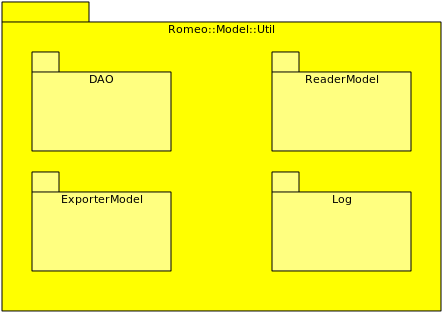
\includegraphics[width=0.8\linewidth]{./Content/Immagini/Romeo__Model__Util.png}
			\caption{Diagramma package \textsl{Romeo::Model::Util}}
			\label{comp_romeo::model::util}
		\end{figure}

		\subsubsection{Descrizione}
		\label{descr_util}
		L'obiettivo di questo package\glossario{} è quello di fornire una serie di classi di utilità e di supporto per le funzionalità core dell'applicativo.
		\subsubsection{Package contenuti}
		\label{pack_util}
		\begin{itemize}
			\item \hyperref[romeo::model::util::dao]{Romeo::Model::Util::DAO};
			\item \hyperref[romeo::model::util::exportermodel]{Romeo::Model::Util::ExporterModel};
\item \hyperref[romeo::model::util::readermodel]{Romeo::Model::Util::ReaderModel};
			\item \hyperref[romeo::model::util::log]{Romeo::Model::Util::Log}.
		\end{itemize}
\pagebreak
%%%%%%%%%%%%%%%%%%%%%%%%%%%%%%%%%%%%%%%%%%%%	
% 		DAO
%%%%%%%%%%%%%%%%%%%%%%%%%%%%%%	
	\subsection{Romeo::Model::Util::DAO}
	\label{romeo::model::util::dao}
		\subsubsection{Informazioni sul package}
		\label{info_dao}
		\begin{figure}[!h]
			\centering
			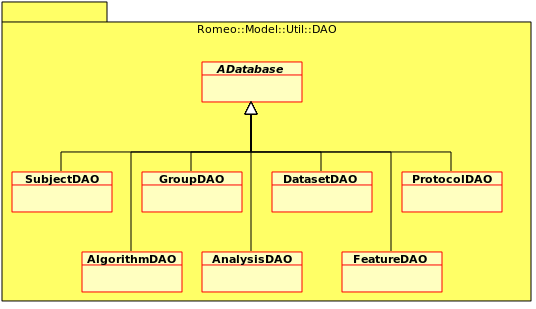
\includegraphics[width=\linewidth]{./Content/Immagini/DAO.png}
			\caption{Diagramma package \textsl{Romeo::Model::Util::DAO}}
			\label{comp_romeo::model::util::dao}
		\end{figure}
		\subsubsection{Descrizione}
		\label{descr_dao}
		Package\glossario{} che gestisce l'interfacciamento con il database del sistema\footnote{Per maggiori informazioni vedere la sezione \ref{DB}}.
		\\Per ogni tabella del database è stata creata un una classe che estende la classe astratta \hyperref[dao::adatabase]{ADatabase}.
		
		\subsubsection{Classi contenute}
		\paragraph{\underline{ADatabase}}
		\label{dao::adatabase} 
		
			\subparagraph{Descrizione:} classe astratta che fornisce i metodi di connessione e disconnessione al database e dei metodi per notificare eventuali errori dovuti al collegamento con componenti esterne, nel nostro caso, il database. Tale classe viene solamente estesa dalle classi che opereranno sulle tabelle del database.
			
			\subparagraph{Utilizzo:} la classe viene creata alla creazione di una sua sottoclasse.
			
			\subparagraph{Eredita da:}
				\begin{itemize}
					\item \hyperref[]{Qt::QSqlDatabase}.
				\end{itemize}
			\subparagraph{Ereditata da:}
				\begin{itemize}
					\item \hyperref[dao::subjectdao]{Romeo::Model::Util::DAO::SubjectDAO};
					\item \hyperref[dao::groupdao]{Romeo::Model::Util::DAO::GroupDAO};
					\item \hyperref[dao::datasetdao]{Romeo::Model::Util::DAO::DatasetDAO};
					\item \hyperref[dao::protocoldao]{Romeo::Model::Util::DAO::ProtocolDAO};
					\item \hyperref[dao::algorithmdao]{Romeo::Model::Util::DAO::AlgorithmDAO};
					\item \hyperref[dao::analysisdao]{Romeo::Model::Util::DAO::AnalysisDAO};
					\item \hyperref[dao::featuredao]{Romeo::Model::Util::DAO::FeatureDAO}.
				\end{itemize}
				
		\paragraph{\underline{SubjectDAO}}
		\label{dao::subjectdao}
		
			\subparagraph{Descrizione:} classe che rappresenta l’oggetto incaricato di operare con la tabella Subject\g{} del database.
 			
 			\subparagraph{Utilizzo:} la classe verrà utilizza quando di dovrà salvare nel database, o recuperare da esso informazioni riguardanti i Subject\g{} creati dall'utente o utilizzati da Romeo\g{}.
 			
			\subparagraph{Eredita da:}
				\begin{itemize}
					\item \hyperref[romeo::model::util::dao]{Romeo::Model::Util::DAO::ADatabase}.		
				\end{itemize}
				
			\subparagraph{Relazioni con altre classi:}
				\begin{itemize}
					\item \hyperref[]{Romeo::Model::Core::ASubject:} relazione uscente, la classe \textsl{SubjectDAO} necessita del tipo \textsl{ASubject} per la sua implementazione;
					
					\item \hyperref[]{Romeo::Model::Core::ProxySubject:} relazione uscente, la classe \textsl{SubjectDAO} necessita del tipo \textsl{ProxySubject} per la sua implementazione:
					
					\item \hyperref[]{Romeo::Controller::NewSubjectController:} relazione entrante, la classe \textsl{NewSubjectController} utilizza \textsl{SubjectDAO} per la creazione di nuovi Subject\g{} in Romeo\g{};
					
					\item \hyperref[]{Romeo::Controller::SubjectsController:} relazione entrante, la classe \textsl{SubjectsController} utilizza \textsl{SubjectDAO} per ottenere la lista di Subject\g{} presenti nel sistema.
					
				\end{itemize}
		
		\paragraph{\underline{GroupDAO}}
		\label{dao::groupdao}
			\subparagraph{Descrizione:} classe che rappresenta l’oggetto incaricato di operare con la tabella GroupOfSubject del database.
			
			\subparagraph{Utilizzo:} la classe verrà utilizza quando si dovrà salvare nel database, o recuperare da esso informazioni riguardanti i Gruppi di Subject creati dall'utente o utilizzati da Romeo\g{}.
			
			\subparagraph{Eredita da:}
				\begin{itemize}
					\item \hyperref[romeo::model::util::dao]{Romeo::Model::Util::DAO::ADatabase}.			
				\end{itemize}
				
			\subparagraph{Relazioni con altre classi:}
				\begin{itemize}
					\item \hyperref[]{Romeo::Model::Core::GroupOfSubject:} relazione uscente, la classe \textsl{SubjectDAO} necessità del tipo \textsl{GroupOfSubject} per la sua implementazione;
					
					\item \hyperref[]{Romeo::Controller::NewGroupController:} relazione entrante, la classe \textsl{NewGroupController} utilizza \textsl{GroupOfSubject} per creare un nuovo gruppo di Subject\g{} in Romeo\g{};
					
					\item \hyperref[]{Romeo::Controller::GroupsController:} relaizone entrante, la classe \textsl{GroupsController} utilizza \textsl{GroupOfSubject} per visualizzare i gruppi di Subject\g{} esistenti.
				\end{itemize}
				
		\paragraph{\underline{ProtocolDAO}}
			\label{dao::protocoldao} 
			
				\subparagraph{Descrizione:} classe che rappresenta l’oggetto incaricato di operare con la tabella Protocol del database.
				
				\subparagraph{Utilizzo:} la classe verrà utilizzata quando si dovrà salvaere nel database, o recupare da esso informazioni riguardanti i Protocol\g{} creati dall'utente o utilizzati da Romeo\g{}.
				
				\subparagraph{Eredita da:}
					\begin{itemize}
						\item \hyperref[romeo::model::util::dao]{Romeo::Model::Util::DAO::ADatabase}.			
					\end{itemize}
					
				\subparagraph{Relazioni con altre classi:}
					\begin{itemize}
					
						\item \hyperref[]{Romeo::Model::Core::Protocol:} relazione uscente, la classe \textsl{ProtocolDAO} necessità del tipo \textsl{Protocol} per la sua implementazione;
						
						\item \hyperref[]{Romeo::Controller::NewProtocolController:} relazione entrante, la classe \textsl{NewProtocolController} utilizza \textsl{Protocol} per creare nuovi Protocol\g{} in Romeo\g{};
						
						\item \hyperref[]{Romeo::Controller::ProtocolsController:} relazione entrante, la classe \textsl{ProtocolsController} utilizza \textsl{Protocol} per visualizzare i \textsl{Protocol} presenti in Romeo\g{}.
					\end{itemize}
				
		\paragraph{\underline{DatasetDAO}}
		\label{dao::datasetdao} 
		
			\subparagraph{Descrizione:}  classe che rappresenta l’oggetto incaricato di operare con la tabella Protocol del database.
			
			\subparagraph{Utilizzo:} la classe verrà utlizzata quando si dovrà salvare nel database, o recuperare da esso informazioni riguardanti i Dataset\g{} creati dall'utente o utilizzati da Romeo\g{}.
							
			\subparagraph{Eredita da:}
			\begin{itemize}
				\item \hyperref[romeo::model::util::dao]{Romeo::Model::Util::DAO::ADatabase}.			
			\end{itemize}
			
			\subparagraph{Relazioni con altre classi:}
				\begin{itemize}
					
					\item \hyperref[]{Romeo::Model::Core::Dataset:} relazione uscente, la classe \textsl{DatasetDAO} necessità del tipo \textsl{Dataset} per la sua implementazione;
											
					\item \hyperref[]{Romeo::Controller::NewDatasetController:} relazione entrante, la classe \textsl{NewDatasetController} utilizza \textsl{Dataset} per creare nuovi Dataset\g{} in Romeo\g{};
											
					\item \hyperref[]{Romeo::Controller::DatasetsController:} relazione entrante, la classe \textsl{DatasetsController} utilizza \textsl{Dataset} per visualizzare i \textsl{Dataset} presenti in Romeo\g{}.
				\end{itemize}
		
		\paragraph{\underline{AlgorithmDAO}}
		\label{dao::algorithmdao}
				\subparagraph{Descrizione:}  classe che rappresenta l’oggetto incaricato di operare con la tabella Algorithm del database.
				
				\subparagraph{Utilizzo:} la classe verrà utilizzata quando si dovrà salvere nel database, o recuperare da esso informazioni riguardanti gli Algoritmi di Cluster\g{} creati dall'utente o utilizzati da Romeo\g{}.		
								
				\subparagraph{Eredita da:}
				\begin{itemize}
					\item \hyperref[romeo::model::util::dao]{Romeo::Model::Util::DAO::ADatabase}.			
				\end{itemize}
				
				\subparagraph{Relazioni con altre classi:}
					\begin{itemize}
						
						\item \hyperref[]{Romeo::Model::Core::AAlgorithm:} relazione uscente, la classe \textsl{AlgorithmDAO} necessità del tipo \textsl{AAlgorithm} per la sua implementazione;
												
						\item \hyperref[]{Romeo::Controller::NewProtocolController:} relazione entrante, la classe \textsl{NewProtocolController} utilizza \textsl{AlgorithmDAO} per aggiungere un algoritmo di cluster\g{} al Protocol\g{} che l'utente sta creando;
												
						\item \hyperref[]{Romeo::Controller::ProtocolsController:} relazione entrante, la classe \textsl{ProtocolsController} utilizza \textsl{AlgorithmDAO} per ottenere gli algoritmi di cluster\g{} dei vari Protocol\g{} presenti nel sistema.
					\end{itemize}
					
			\paragraph{\underline{FeatureDAO}}
			\label{dao::featuredao} 
				\subparagraph{Descrizione:}  classe che rappresenta l’oggetto incaricato di operare con la tabella Feature del database.
									
				\subparagraph{Utilizzo:} la classe verrà utilizzata quando si dovrà salvare nel database, o recuperare da esso informazioni riguardanti le feature\g{} create dall'utente o utlizzate da Romeo\g{}.	
												
				\subparagraph{Eredita da:}
					\begin{itemize}
						\item \hyperref[romeo::model::util::dao]{Romeo::Model::Util::DAO::ADatabase}.			
					\end{itemize}
								
				\subparagraph{Relazioni con altre classi:}
					\begin{itemize}
						
						\item \hyperref[]{Romeo::Model::Core::AFeature:} relazione uscente, la classe \textsl{FeatureDAO} necessità del tipo \textsl{AAlgorithm} per la sua implementazione;
												
						\item \hyperref[]{Romeo::Controller::NewProtocolController:} relazione entrante, la classe \textsl{NewProtocolController} utilizza \textsl{FeatureDAO} per aggiungere/eliminare le feature\g{} al Protocol\g{} che l'utente sta creando;
												
						\item \hyperref[]{Romeo::Controller::ProtocolsController:} relazione entrante, la classe \textsl{ProtocolsController} utilizza \textsl{AlgorithmDAO} per ottenere le feature\g{} dei vari Protocol\g{} presenti nel sistema.
					\end{itemize}
			
	\paragraph{\underline{AnalysisDAO}}
	\label{dao::analysisdao} 
					\subparagraph{Descrizione:}  classe che rappresenta l’oggetto incaricato di operare con la tabella Analysis del database.
							
					\subparagraph{Utilizzo:} la classe verrà utilizzata quando si dovrà salvare nel database, o recuperare da esso informazioni riguardanti le feature\g{} create dall'utente o utilizzata da Romeo\g{}.				
													
					\subparagraph{Eredita da:}
						\begin{itemize}
							\item \hyperref[romeo::model::util::dao]{Romeo::Model::Util::DAO::ADatabase}.			
						\end{itemize}
									
					\subparagraph{Relazioni con altre classi:}
						\begin{itemize}
							
							\item \hyperref[]{Romeo::Model::Core::Analysis:} relazione uscente, la classe \textsl{AnalyisDAO} necessità del tipo \textsl{Analyisis} per la sua implementazione;
													
							\item \hyperref[]{Romeo::Controller::AnalysisController:} relazione entrante, la classe \textsl{AnalysisController} utilizza \textsl{AnalysisDAO} per avviare una nuova analisi in Romeo\g{};
							
							\item \hyperref[]{Romeo::Controller::ResultsController:} relazione entrante, la classe \textsl{ResultsController} utilizza \textsl{AnalysisDAO} per ottenere la lista di analisi effettuate;
							
							\item \hyperref[]{Romeo::Controller::DetailedResultController:} relazione entrante, la classe \textsl{DetailedResultController} utilizza \textsc{AnalysisDAO} per ottenere i dettagli di una specifica analisi effettuata.						
		
						\end{itemize}
					










\subsection{Romeo::Model::Util::ExporterModel}
	\label{romeo::model::util::exportermodel}
		\subsubsection{Informazioni sul package}
		\label{info_expmod}
		\begin{figure}[!h]
			\centering
			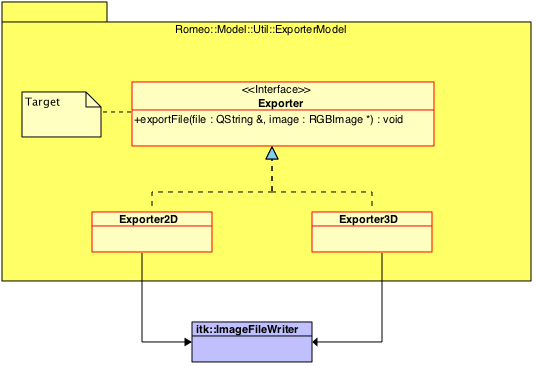
\includegraphics[width=\linewidth]{./Content/Immagini/ExporterModel.png}
			\caption{Package \textsl{Romeo::Model::Util::ExporterModel}}
			\label{comp_log}
		\end{figure}

		\subsubsection{Descrizione}
		\label{descr_expmod}
		Package\g{} contenente le classi che si occupano di trasformare le immagini dal formato interno usato per l'analisi, al formato desiderato dall'utente, tra quelli previsti dai requisiti.
		\\Le classi di questo package\g{} sono implementate tramite il design pattern\g{} Adapter utilizzando le classi fornite dalla libreria esterna ITK\g{}.

		\subsubsection{Interfacce contenute}
		\label{interface_exporter}
			\paragraph{\underline{Exporter}}
			\label{expo}
			 	\subparagraph{Descrizione:} interfaccia che fornisce un contratto per esportare i risultati delle analisi. Viene implementata dalle classi che specializzano l'esportazione per tipologia di file.
			 	\\Rappresenta il componente Target del design pattern\g{} Adapter.
			 	\subparagraph{Utilizzo:} viene implementata dalle classi Exporter2D ed Exporter3D che ne implementano i metodi.
			 	\subparagraph{Implementata da:}
					\begin{itemize}
						\item \hyperref[expo_analyze]{Romeo::Model::Util::ExporterModel::Exporter2D};
						\item \hyperref[expo_img]{Romeo::Model::Util::ExporterModel::Exporter3D}.	
					\end{itemize}

				\subparagraph{Relazioni con altre classi:}
					\begin{itemize}
						\item \hyperref[]{Romeo::Model::Core::Analysis:} relazione entrante, la classe Analysis utilizza l'interfaccia Exporter per esportare i risultati durante l'analisi.
						\item \hyperref[]{Romeo::Model::Core::RGBImage} relazione uscente, l'interfaccia utilizza la classe RGBImage quando deve esportare un'immagine.
					\end{itemize}

		\subsubsection{Classi contenute}
		\label{exporter_contenute}
		\paragraph{\underline{Exporter2D}}
				\label{expo_analyze}
				 	\subparagraph{Descrizione:} classe che si occupa di esportare un immagine di tipo 2D, nel formato desiderato dall'utente tra quelli previsti dai requisiti e nel percorso indicato dall'utente o dal signal\glossario{} che la utilizza.
				\subparagraph{Utilizzo:} la classe viene utilizzata in seguito alla ricezione di un signal\glossario{} da parte dei controller che necessita di esportare un'immagine di tipo 2D. 
				\\Classe che viene utilizzata come adattatore della classe ImageFileWriter, fornita dalla libreria esterna ITK\g{}. Rappresenta il componente Adapter del design pattern\g{} Adapter.
				 	\subparagraph{Eredita da:}
							\begin{itemize}
								\item \hyperref[expo]{Romeo::Model::Util::ExporterModel::Export}.				
							\end{itemize}
					\subparagraph{Relazioni con altre classi:}
						\begin{itemize}
							\item \hyperref[]{Romoe::Model::Core::Analysis:} relazione entrante, la classe Analysis utilizza la classe AnalyzeExporter per esportare i risultati dell'analisi in formato Analyze\g{}.
							\item \hyperref[]{Romeo::Model::Core::RGBImage} relazione uscente, l'interfaccia utilizza la classe RGBImage quando deve esportare un'immagine.
						\end{itemize}

		\paragraph{\underline{Exporter3D}}
			\label{expo_img} 
				\subparagraph{Descrizione:} classe che si occupa di esportare un immagine di tipo Analyze\g{}, nel percorso indicato dall'utente o dal signal\glossario{} che la utilizza. 
				\subparagraph{Utilizzo:} la classe viene utilizzata in seguito alla ricezione di un signal\glossario{} da parte dei controller che necessita di esportare un'immagine di tipo 3D.
				 	\\Classe che viene utilizzata come adattatore della classe ImageFileWriter, fornita dalla libreria esterna ITK\g{}. Rappresenta il componente Adapter del design pattern\g{} Adapter.
				\subparagraph{Eredita da:}
					\begin{itemize}
						\item \hyperref[expo]{Romeo::Model::Util::ExporterModel::Export}.				
					\end{itemize}	
				\subparagraph{Relazioni con altre classi:}
					\begin{itemize}
						\item \hyperref[]{Romoe::Model::Core::Analysis:} relazione entrante, la classe Analysis utilizza la classe ImageExporter per esportare i risultati dell'analisi in un formato immagine generico.
							\item \hyperref[]{Romeo::Model::Core::RGBImage} relazione uscente, l'interfaccia utilizza la classe RGBImage quando deve esportare un'immagine.
						\end{itemize}	


%%%%%%%%%%%%%%%%%%%%%%%%%%%
% 	READERMODEL
%%%%%%%%%%%%%%%%%%%%%%%%%%%		
	\pagebreak
		\subsection{Romeo::Model::Util::ReaderModel}
	\label{romeo::model::util::readermodel}
		\subsubsection{Informazioni sul package}
		\label{info_readmod}
		\begin{figure}[!h]
			\centering
			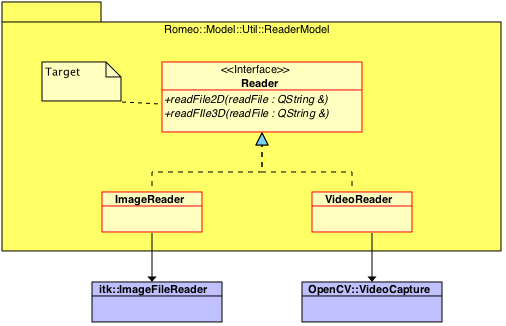
\includegraphics[width=0.9\linewidth]{./Content/Immagini/Romeo__Model__Util__ReaderModel.png}
			\caption{Pacakge \textsl{Romeo::Model::Util::ReaderModel}}
			\label{comp_read}
		\end{figure}
		\subsubsection{Descrizione:}
		\label{descr_readmod}
		Package\g{} contenente le classi che si occupano di leggere le immagini e trasformarle nel formato interno usato all'interno di \project{}.
		\\Le classi di questo package\g{} sono implementate tramite il design pattern\g{} Adapter adattando le classi fornite dalla libreria esterna ITK\g{}.


		\subsubsection{Interfacce contenute}
		\label{interface_readere}
			\paragraph{\underline{Reader}}
			\label{reader}
				\subparagraph{Descrizione:} interfaccia che fornisce un contratto per la lettura di immagini e la trasformazione di esse nel formato interno. Viene implementata dalle classi che specializzano la lettura per tipologia di file.
				\\Rappresenta il componente Target del design pattern\g{} Adapter.
				\subparagraph{Utilzzo:} viene implementata dalle classi ImageReader e VideoReader che ne implementano i metodi.				
				\subparagraph{Implementata da:}
					\begin{itemize}
						\item \hyperref[rea_img]{Romeo::Model::Util::ReaderModel::ImageReader};	
						\item \hyperref[rea_video]{Romeo::Model::Util::ReaderModel::VideoReader}.
					\end{itemize}
				\subparagraph{Relazioni con altre classi:}
					\begin{itemize}
						\item \hyperref[]{Romeo::Model::Core::RealSubject:} relazione entrante, la classe RealSubject necessità dell'interfaccia Reader per la sua implementazione.
					\end{itemize}

				\pagebreak

		\paragraph{\underline{ImageReader}}
		\label{rea_img}
			\subparagraph{Descrizione:} classe che si occupa di caricare immagini di tipo 2D e 3D non time dipendent. Viene utilizzata come adattatore dalla classe \verb!ImageFileReader! fornita dalla libreria esterna ITK\g{}.
			\\Rappresenta il componente Adapter del design pattern\g{} Adapter.
			\subparagraph{Utilizzo:} viene utilizzata quando c'è necessità di operare sull'immagine, quindi durante l'analisi e durante la creazione dei subject.
			\subparagraph{Eredita da:}
				\begin{itemize}
					\item \hyperref[reader]{Romeo::Model::Util::ReaderModel::Reader}.
				\end{itemize}
			\subparagraph{Relazioni con altre classi:}
					\begin{itemize}
						\item \hyperref[]{Romeo::Model::Core::RGBImage:} relazione entrante, la classe RGBImage necessità della classe ImageReader per la sua implementazione;
						\item \hyperref[]{Romeo::Model::Core::RBGImage2D:} relazione entrante, la classe RGBImage2D necessità della classe ImageReader per la sua implementazione.					
						\item \hyperref[]{Romeo::Model::Core::RGBImage3D:}	relazione entrante, la classe RGBImage3D necessità della classe ImageReader per la sua implementazione.					
						\item \hyperref[]{Romeo::Model::Core::InternalData2D:}	relazione entrante, la classe InternalData2D necessità della classe ImageReader per la sua implementazione.
						\item \hyperref[]{Romeo::Model::Core::InternalData3D:}	relazione entrante, la classe InternalData3D necessità della classe ImageReader per la sua implementazione.						
					\end{itemize}

		\paragraph{\underline{VideoReader}}
		\label{rea_video}
			\subparagraph{Descrizione:} classe che si occupa di caricare video di tipo 2D e 3D. Classe che viene utilizzata come adattatore della classe \verb!VideoFileReader! fornita dalla libreria
			esterna ITK\g{}.
			\\Rappresenta il componente Adapter del design pattern\g{} Adapter.
			\subparagraph{Utilizzo:} viene utilizzata quando c'è necessità di operare sui video, quindi durante l'analisi e durante la creazione dei subject.
			\subparagraph{Eredita da:}
				\begin{itemize}
					\item \hyperref[reader]{Romeo::Model::Util::ReaderModel::Reader}.
				\end{itemize}
			\subparagraph{Relazioni con altre classi:}
				\begin{itemize}
						\item \hyperref[]{Romeo::Model::Core::Video:} relazione entrante, la classe Video necessità della classe VideoReader per la sua implementazione;
						\item \hyperref[]{Romeo::Model::Core::Video2D:} relazione entrante, la classe Video2D necessità della classe VideoReader per la sua implementazione.					
						\item \hyperref[]{Romeo::Model::Core::Video3D:}	relazione entrante, la classe Video3D necessità della classe VideoReader per la sua implementazione.										
				\end{itemize}
				\pagebreak




%%%%%%%%%%%%%%%%%%%%%%%%%%
% 		LOG
%%%%%%%%%%%%%%%%%%%%%%%%%%		
	\subsection{Romeo::Model::Util::Log}
	\label{romeo::model::util::log}
		\subsubsection{Informazioni sul package}
		\label{info_log}
		\begin{figure}[!h]
			\centering
			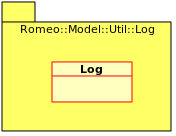
\includegraphics[width=0.6\linewidth]{./Content/Immagini/Romeo__Model__Util__Log.png}
			\caption{Diagramma package\g{} \textsl{Romeo::Model::Util::Log}}
			\label{comp_log}
		\end{figure}
		\subsubsection{Descrizione}
		\label{descr_log}
		Package\g{} contenente la classe che si occupa di gestire e produrre dei file di log, nei quali saranno contenute informazioni utili agli sviluppatori.
		
		\subsubsection{Classi contenute}
		
		\paragraph{\underline{Log}}
		\label{log_class}
			\subparagraph{Descrizione:} classe che si occupa di produrre e scrivere il file di log, con alcune operazioni che \project{} effettuerà. Nel file saranno quindi memorizzate informazioni riguardanti errori derivati dall'uso del programma, azioni dell'utente, esecuzione di analisi e interazione del sistema con il database. 		
			\pagebreak
			
		
		\subsection{Romeo::Model::qtModel}
			\label{romeo::model::qtmodel}
				\subsubsection{Informazioni sul package}
				\label{qtmodel_info}
				\begin{figure}[!h]
					\centering
					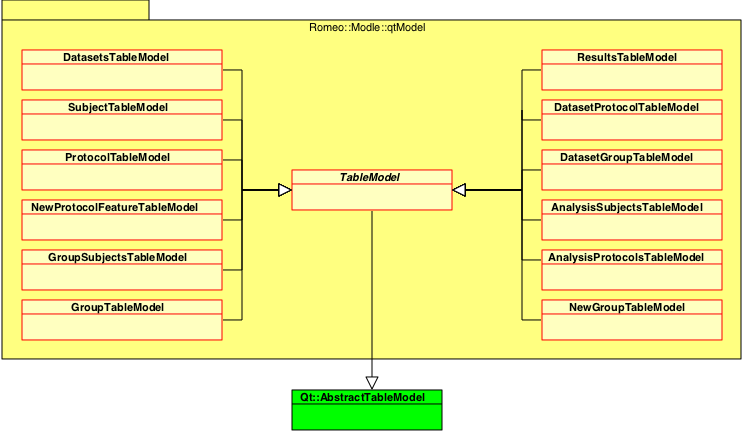
\includegraphics[width=\linewidth]{./Content/Immagini/Romeo__Model__qtModel.png}
					\caption{Diagramma package \textsl{Romeo::Model::qtModel}}
					\label{comp_qtModel}
				\end{figure}
				\subsubsection{Descrizione}
					\label{qtmodel_desc}
					Package\g{} contenente le classi che estendono i Model per le tabelle e liste proprietari di Qt\g{}, utilizzate delle \textsl{QTableView} e \textsl{QListView} presenti nelle view.
					
				\subsubsection{Classi contenute}
						
					\paragraph{\underline{TableModel}}
					\label{TableModel_class}
						\subparagraph{Descrizione:} classe astratta che fornisce un contratto per la generazione del model Qt\g{} per le QTableView.
						
						\subparagraph{Eredita da:}
							\begin{itemize}
								\item Qt::QAbstractTableModel.		
							\end{itemize}
						
						\subparagraph{Ereditata da:}
							\begin{itemize}
								\item Romeo::Model::qtModel::DatasetsTableModel;
								\item Romeo::Model::qtModel::SubjectTableModel;
								\item Romeo::Model::qtModel::ProtocolTableModel;
								\item Romeo::Model::qtModel::NewProtocolFeatureTableModel;
								\item Romeo::Model::qtModel::GroupSubjectsTableModel;
								\item Romeo::Model::qtModel::GroupTableModel;
								\item Romeo::Model::qtModel::ResultsTableModel;
								\item Romeo::Model::qtModel::DatasetProtocolTableModel;
								\item Romeo::Model::qtModel::DatasetGroupTableModel;
								\item Romeo::Model::qtModel::AnalysisSubjectsTableModel;
								\item Romeo::Model::qtModel::AnalysisProtocolsTableModel;
								\item Romeo::Model::qtModel::NewGroupTableModel.
							\end{itemize}
							
		
		%%%%%%%%%%%%%%%%%%%%%%%%%%%%%%%
		% 	help
		%%%%%%%%%%%%%%%%%%%%%%%%%%%%%	
	\subsection{Romeo::Model::Help}
	\label{romeo::model::Help}
		\subsubsection{Informazioni sul package}
		\label{info_help}
		\begin{figure}[!h]
			\centering
			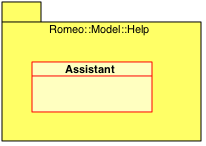
\includegraphics[width=0.6\linewidth]{./Content/Immagini/Help.png}
			\caption{Diagramma package \textsl{Romeo::Model::Help}}
			\label{comp_help}
		\end{figure}
		\subsubsection{Descrizione}
		\label{descr_help}
		Packag\g{} contenente la classe dedicata a caricare il contenuto dei file riguardanti la guida utente.
	
	\subsubsection{Classi contenute}	
		\paragraph{\underline{Assistant}}
		\label{help}
			\subparagraph{Descrizione:} classe che rappresenta il processo Qt Assistant, utilizzato per la gestione della guida utente.
		 	
		 	\subparagraph{Utilizzo:}
		 	 viene utilizzata per gestire la richiesta dell'utente, che vuole visualizzare una determinata pagina all'interno della guida utente.
		 	 
		 	 \subparagraph{Eredita da:}
		 	 		\begin{itemize}
		 	 			\item Qt::QProcess
		 	 		\end{itemize}
		 	 
		 	 \subparagraph{Relazioni con altre classi:}
		 	 	\begin{itemize}
			 	 	\item \hyperref[]{Romeo::Controller::MainWindowController:} relazione entrante, la classe MainWindowController utilizza la classe per avviare la guida utente.
		 	 	\end{itemize}
		 	 	
		 	